\documentclass{article}
\usepackage{authblk}

\usepackage{graphicx}% Include figure files
\usepackage{dcolumn}% Align table columns on decimal point
\usepackage{amsmath,amssymb}
\usepackage{bm}% bold math
\usepackage{enumitem}

\usepackage{hyperref}%to have clickable links
\hypersetup{
    colorlinks=true,
    linkcolor=blue,
    filecolor=magenta,      
    urlcolor=cyan,
}

%\usepackage{geometry}
 
% \geometry{a4paper,total={170mm,257mm},left=25mm, top=25mm, }

\usepackage{afterpage}

%%%%%%%%%%%%%%%%%%%%%%%%%%%%%%%%%%%%%%%%%%%%%%%%%

\title{Multi-class classification on gene expression data}
\author[1]{Simone Daniotti}
\author[2]{Riccardo Castelli}

\affil[1]{Physics Department, University of Milan}
\affil[2]{Informatics Department, University of Milan}
\date{September 26, 2019}                     %% if you don't need date to appear
\setcounter{Maxaffil}{0}
\renewcommand\Affilfont{\itshape\small}

%%%%%%%%%%%%%%%%%%%%%%%%%%%%%%%%%%%%%%%%%%%%%%%%%%%%

\begin{document}

  \maketitle
  

\begin{abstract}
Your abstract goes here...
...
\end{abstract}



\tableofcontents
\newpage


%%%%%%%%%%%%%%%%%%%%%%%%%%%%%%%%%%%%%%%%%%%%%%%%%%%%%%%
%%%%%%%%%%%%%%%%%%%%%%%%%%%%%%%%%%%%%%%%%%%%%%%%%%%%%%%
%%%%%%%%%%%%%%%%%%%%%%%%%%%%%%%%%%%%%%%%%%%%%%%%%%%%%%%


\section{Dataset description}

The dataset for this work is taken from UCI Machine Learning Repo (available at \url{https://archive.ics.uci.edu/ml/datasets/gene+expression+cancer+RNA-Seq}) \cite{Dua:2019}; this is part of the RNA-Seq (HiSeq, a tool for measuring gene expression levels) PANCAN data set. It is a collection of gene expression levels of patients having different types of tumor: BRCA(breast), KIRC(kidney), COAD(colon), LUAD(lung) and PRAD(prostate).
These data represent the quantity of gene information used in the synthesis of a functional gene product. For further information, we refer to \cite{weinstein2013cancer}.


%%%%%%%%%%%%%%%%%%%%%%%%%%%%%%%%%%%%%%%%%%%%%%%
%%%%%%%%%%%%%%%%%%%%%%%%%%%%%%%%%%%%%%%%%%%%%%%%%%%%%%%
%%%%%%%%%%%%%%%%%%%%%%%%%%%%%%%%%%%%%%%%%%%%%%%%%%%%%%%


\section{Dataset Manipulation}


\subsection{Preliminary manipulation}
Both dataset and labels can be downloaded in a csv ('comma separated value') format, then can be easily imported in a Pandas Dataframe (\url{https://pandas.pydata.org/}). The first column represents patient's ID: it has been removed because it is useless for our purposes.

%%%%%%%%%%%%%%%%%%%%%%%%%%%%%%%%%%%%%%%%%%%%%%%%%%%%%%%
%%%%%%%%%%%%%%%%%%%%%%%%%%%%%%%%%%%%%%%%%%%%%%%%%%%%%%%

\subsection{Label handling}
The labels are strings representing the five types of cancer. Learning models can be created using raw features(in the case of trees and forests), using Label Encoding or One-hot Encoding.
Label Encoding creates a map between the string and an ordered sequence of natural numbers, from 0 to 4 in our case.
One-hot encoding creates a single binary label for each class, changing the task of the learning model to a multi-label problem.

%%%%%%%%%%%%%%%%%%%%%%%%%%%%%%%%%%%%%%%%%%%%%%%%%%%%%%%
%%%%%%%%%%%%%%%%%%%%%%%%%%%%%%%%%%%%%%%%%%%%%%%%%%%%%%%


\subsection{Train and Test Set}

For training the net and then evaluating it, we split the dataset in training and test set using the Sklearn library $train\_test\_split$ (\url{https://scikit-learn.org/stable/modules/generated/sklearn.model_selection.train_test_split.html}). We set the seed of the random split and the proportions between the two sets: test set is $0.15$ of the entire database.

%%%%%%%%%%%%%%%%%%%%%%%%%%%%%%%%%%%%%%%%%%%%%%%%%%%%%%%
%%%%%%%%%%%%%%%%%%%%%%%%%%%%%%%%%%%%%%%%%%%%%%%%%%%%%%%

\subsection{Class Weighting}
Since our dataset is unbalanced, we chose to utilise the $class\_weight$ parameter (present in almost every classifier) to handle this problem. This parameter can be defined as a dictionary that maps each class in the dataset with its respective weight; weights can be computed using Scikit-learn method compute class weight in the $class\_weight$ library, which assigns greater values to the less represented classes. Through this parameter, the classifier is aware of the fact that some classes are more represented than others and gives the examples different importance during the training step.
%(https://scikit-learn.org/stable/modules/generated/sklearn.utils.class_weight.compute_class_weight.html)
%%%%%%%%%%%%%%%%%%%%%%%%%%%%%%%%%%%%%%%%%%%%%%%
%%%%%%%%%%%%%%%%%%%%%%%%%%%%%%%%%%%%%%%%%%%%%%%%%%%%%%%
%%%%%%%%%%%%%%%%%%%%%%%%%%%%%%%%%%%%%%%%%%%%%%%%%%%%%%%


\section{Architectures}
There are lots of books reviewing these architectures and concepts. Here we refer to \cite{geron2017hands} , \cite{bishop2006pattern} \cite{hertz1991introduction}.

%%%%%%%%%%%%%%%%%%%%%%%%%%%%%%%%%%%%%%%%%%%%%%%%%%%%%%%
%%%%%%%%%%%%%%%%%%%%%%%%%%%%%%%%%%%%%%%%%%%%%%%%%%%%%%%

\subsection{Support Vector Machines (SVM)}
Another approach that we used to create a model that well classifies our dataset is the Support Vector Machines (or SVM in short). Both a binary and a multi-class classifier, SVM tries to find the hyperplane, called decision boundary, that best separates the data. The optimal hyperplane is chosen by the use of the so called “support vectors”, which are the samples of each class closest to the hyperplane. The distance between the support vectors is called margin, and the goal of the SVM is to maximise this margin in order to get a good separation between the classes in a way that also guarantees a good generalisation. 
SVM are particularly effective in high dimensional spaces, even when the number of features is greater than the number of samples; as this fact fits very well with the properties of our dataset, we decided to experiment the classification with this kind of model to see the results. 
For the implementation, we utilised Scikit-learn SVC class from the svm library: for multi-class classification, it uses a “one-against-one” approach, creating $[n_class*(n\_class-1)/2]$ classifiers and train each of them with two classes. We considered three parameters for our model: C, kernel and $class\_weights$. 
C is called the ‘soft margin constant’: we can describe it as a measure of tolerance regarding the misclassification of the data, the more the C increases, the less amount of misclassified points the model will tolerate, and during the training process it will try find a trade-off between the maximisation of the margin and the minimisation of the misclassification. 
Kernel are used by the SVM to apply transformations to the data in order to project them in a higher dimensional space where they are more likely to be separable; this method, called the “kernel trick” is used to find non-linear decision boundaries. 
The parameter $class\_weights$ is used to make the SVM aware that the dataset is unbalanced. 

%%%%%%%%%%%%%%%%%%%%%%%%%%%%%%%%%%%%%%%%%%%%%%%%%%%%%%%
%%%%%%%%%%%%%%%%%%%%%%%%%%%%%%%%%%%%%%%%%%%%%%%%%%%%%%%

\subsection{Decision Tree Classifier and Random Forests}

Decision Trees are versatile Machine Learning algorithms that can perform both classification and regression tasks, and even multioutput tasks. They are particularly useful in treating with complex data, such as a dataset that can hardly be represented by a vector in a multi-dimensional space: this is not our case, but we think it is useful to approach our problem with more simple models and evaluating them before \textit{deeping} in more difficult models.
Tree Classifiers have the structure of an \textit{ordered and rooted tree}. It is \textit{ordered} because the children of any internal node are numbered consecutively, and \textit{rooted} because splitting starts from only one node.
From that node, the model is built following the attribute selection measure.
Attribute selection measure is a heuristic for selecting the splitting criterion that partition data into the best possible manner.

\begin{figure}[h!]
\centering
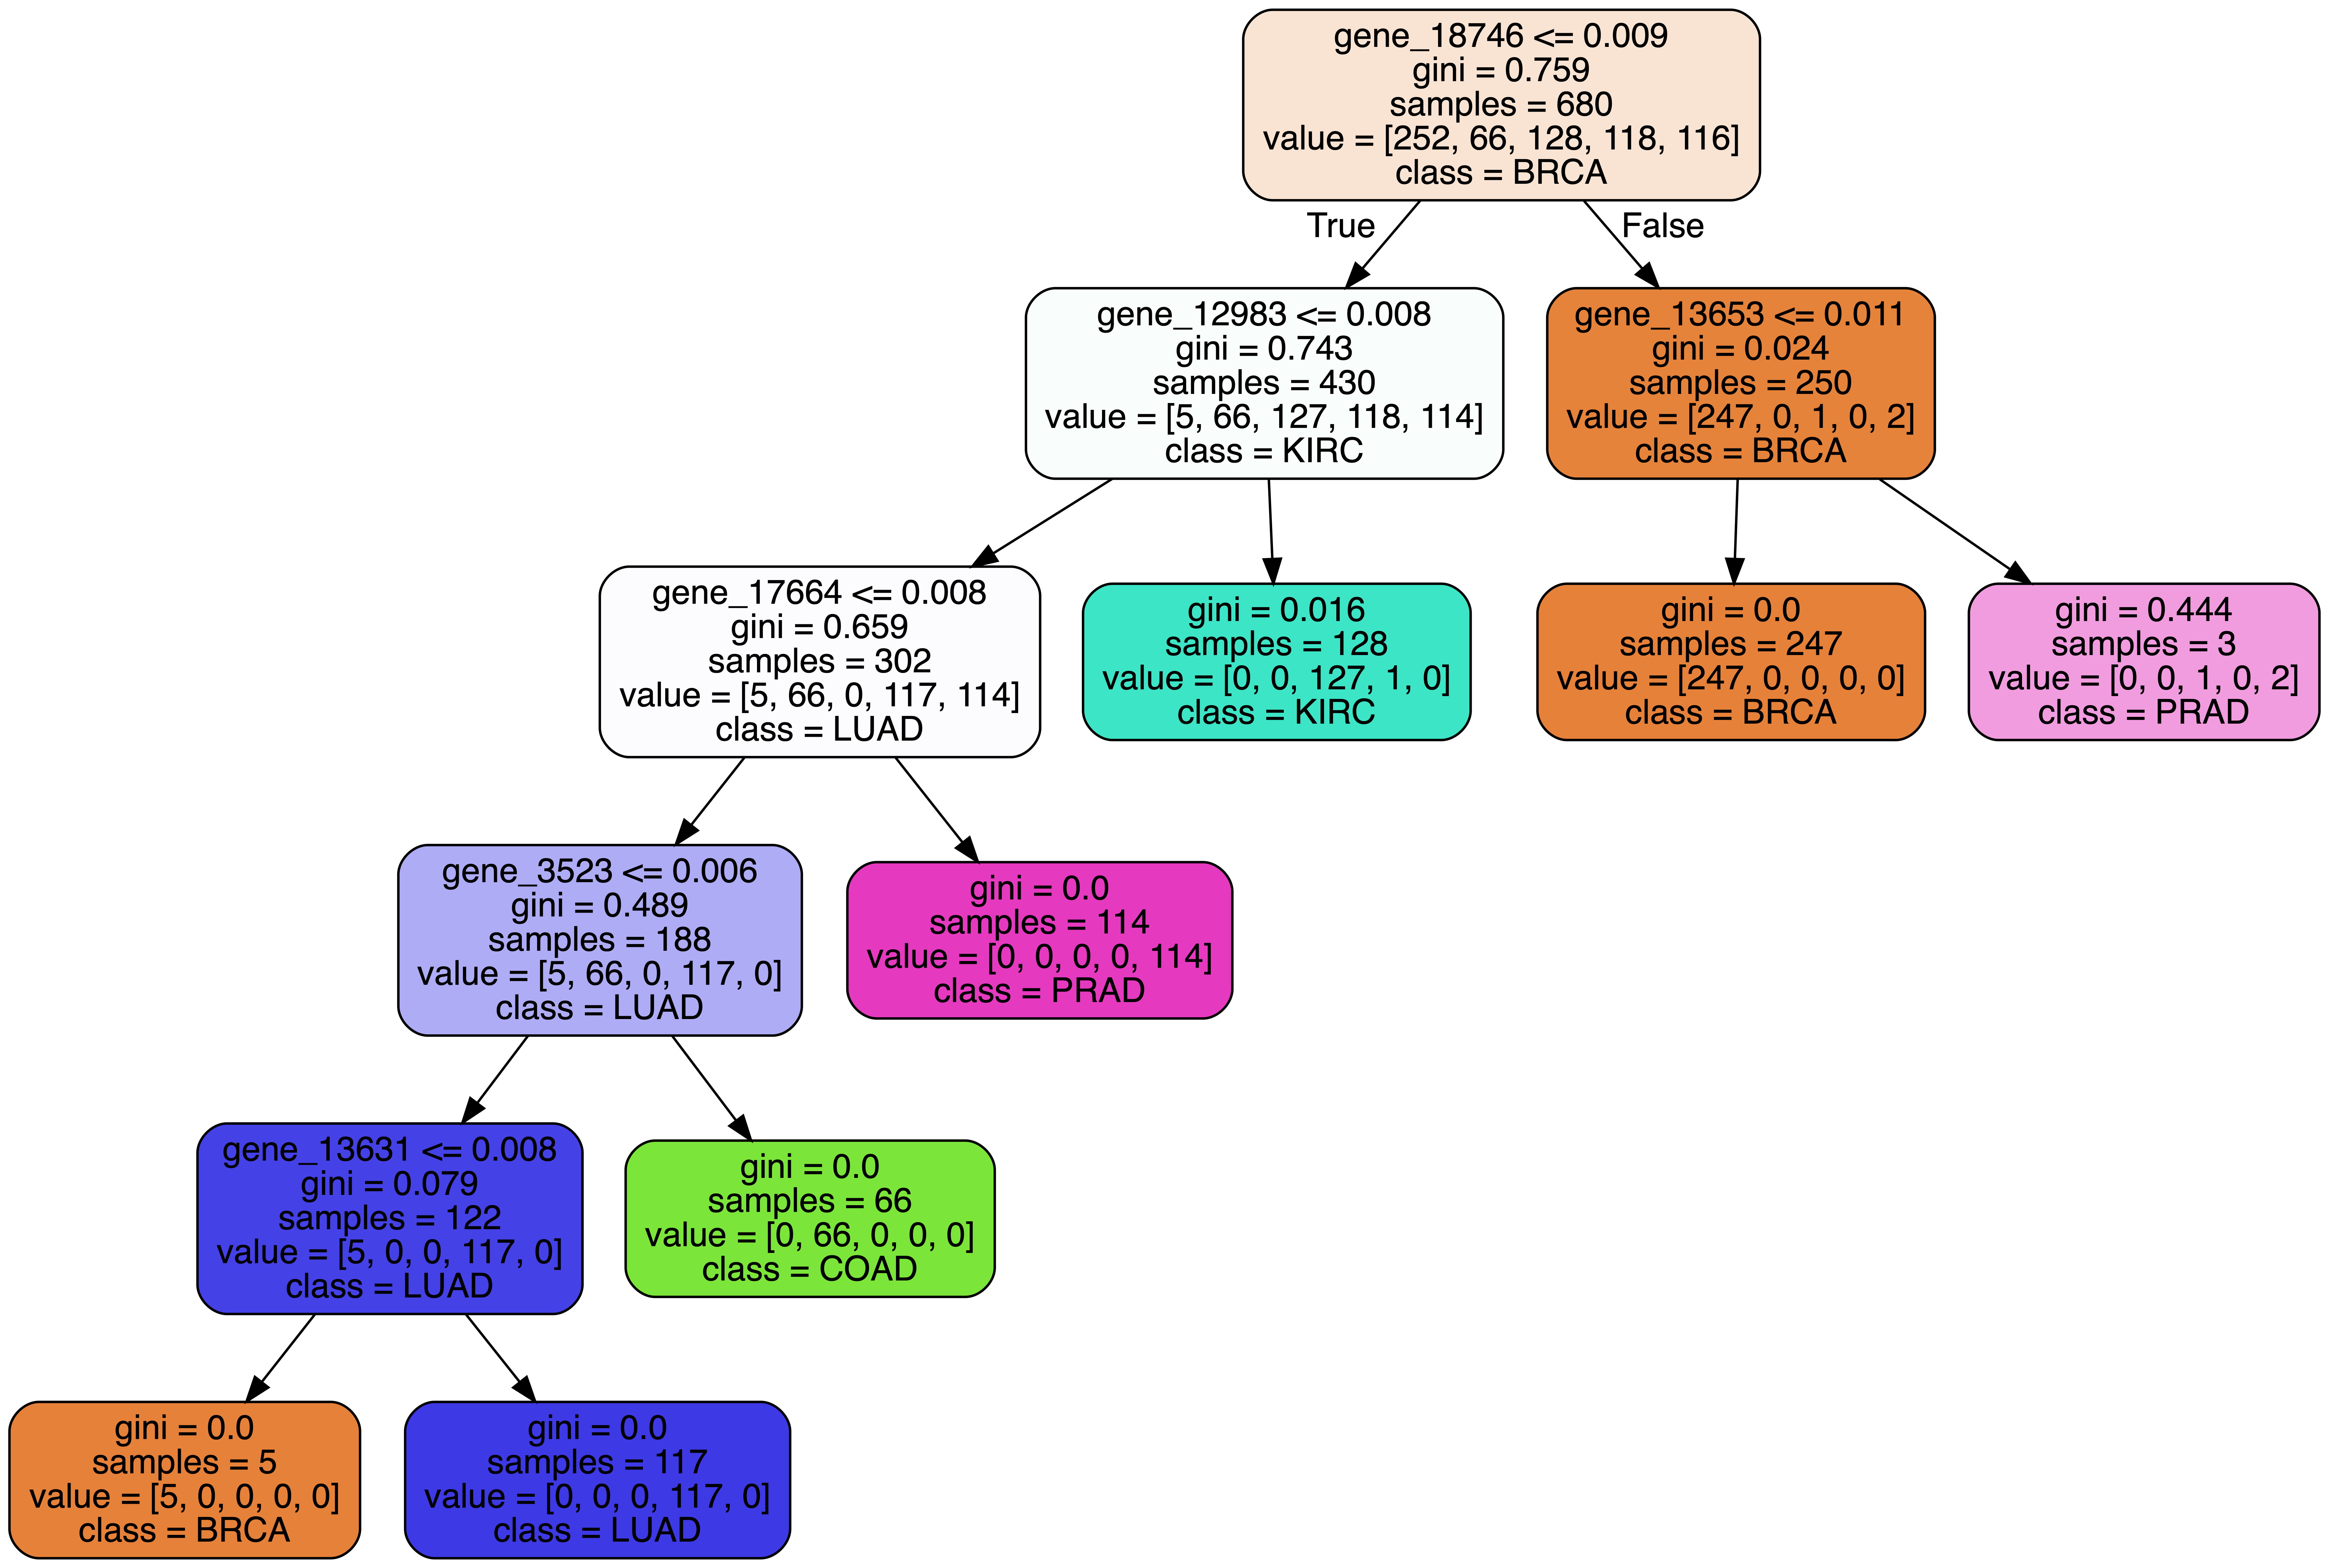
\includegraphics[width=\linewidth]{img/tree_best.png}
\caption{Shape of a tree classifier, with hyperparameters tuned by tecniques explained below.}
\label{fig1}
\end{figure}


Scikit-Learn uses the \textit{Classification And Regression Tree (CART) algorithm} to train Decision Trees.It works as follows: it first splits the training set in two subsets using a single feature k and a threshold $t_k$ . How does it choose $k$ and $t_k$? It searches for the pair $(k, t_k)$ that produces the purest subsets. The cost functions that the algorithm tries to minimize are different: most used are \textit{Gini Impurity} and \textit{Entropy}, tunable in Scikit-learn by the hyperparameter \textit{criterion}. Entropy hyperparameter measures Shannon's Entropy, a concept taken from information theory.
Each leaf of the tree corresponds to a possible classification label, so inserting datas of a patient from the root, the model $spits$ its classification. This can be a modality for building a predictor.


If you aggregate the predictions of a group of predictors (regulated by certain rules, such as majority rule..), you will often get better predictions than with the best individual predictor. A group of predictors is called an \textit{ensemble}; thus, this technique is called \textit{Ensemble Learning}, and an Ensemble Learning algorithm is called an \textit{Ensemble method}.
Training a group of Decision Tree Classifiers and gathering into one single predictor is called a \textit{Random Forest}.
The Random Forest algorithm introduces extra randomness when growing trees; instead of searching for the very best feature when splitting a node (as in the tree case), it searches for the best feature among a random subset of features. This results in a greater tree diversity.


%%%%%%%%%%%%%%%%%%%%%%%%%%%%%%%%%%%%%%%%%%%%%%%%%%%%%%%
%%%%%%%%%%%%%%%%%%%%%%%%%%%%%%%%%%%%%%%%%%%%%%%%%%%%%%%

\subsection{Deep Learning}

PARTE MANCANTE, DA FARE IN SEGUITO
%%%%%%%%%%%%%%%%%%%%%%%%%%%%%%%%%%%%%%%%%%%%%%%%%%%%%%%

\subsubsection{PyTorch}

PyTorch is a Python machine learning framework. It is built for creating learning algorithms based on graph models. 
It starts as a low-level library, but has a lot of high-level APIs for building big deep neural network in a bunch of code lines.
Its core element are Pytorch tensors, in the same way arrays are for Numpy, but are build to take advantage of GPU computing in an easy way.
Transition between low-level programming and APIs is truly continuous: this is a very important feature in building and tweaking a Deep Neural Network.
In depth, it has some useful built-in methods to handle training and evaluation, for example: autograd() to compute gradients and DataLoader() to handle training and batch loading.
All further documentation can be found here: \url{https://pytorch.org/}.
%%%%%%%%%%%%%%%%%%%%%%%%%%%%%%%%%%%%%%%%%%%%%%%%%%%%%%%

\subsubsection{Keras}
Keras is a Python high-level machine learning library capable of running on top of multiple back-ends (such as TensorFlow, Theano, CNTK and many more), taking advantage of their power but putting aside their complexity. In fact, Keras allows the user to build deep learning models through a long list of modules that can be selected and combined in a very easy to use manner, which does not however comes at the expenses of the flexibility of the back-end frameworks and does not limit the user during the development and implementation process. 
The main Keras model is the Sequential, which is a linear stack of layers. The construction of the model requires three main phases: adding layers, compile the model and train it. 
In the first phase we can add an arbitrary number of layers using the add function. There is a consistent number of type of layers that can be selected, for example, in our model, we chose to use 3 Dense (that is fully-connected) layers and 3 Dropout layers for regularization purposes. 
The second phase is where the model is compiled through the compile function; the function needs the optimizer, the loss function and the metrics of evaluation to be specified. 
The third and last phase is the training of the model: Keras uses the fit function for this purpose, to which we have to pass for example (other than the training examples and labels) the batch size, the epochs and the class weights. 
After the model has been built and trained, it can be evaluated on the test set using Keras’ method evaluate.

%%%%%%%%%%%%%%%%%%%%%%%%%%%%%%%%%%%%%%%%%%%%%%%
%%%%%%%%%%%%%%%%%%%%%%%%%%%%%%%%%%%%%%%%%%%%%%%%%%%%%%%
%%%%%%%%%%%%%%%%%%%%%%%%%%%%%%%%%%%%%%%%%%%%%%%%%%%%%%%


\section{Parameter optimization and Validation}

Once having built the net, a user must ensure that the model has a good generalizing capacity. Often, a too fitted net fails to predict in test set, in a sense longly described in the books cited above; this behaviour is called \textit{overfitting}.
In the sections below, we will review some of the tecniques used to avoid this feature and some characteristics of the models we studied.
%%%%%%%%%%%%%%%%%%%%%%%%%%%%%%%%%%%%%%%%%%%%%%%%%%%%%%%
%%%%%%%%%%%%%%%%%%%%%%%%%%%%%%%%%%%%%%%%%%%%%%%%%%%%%%%

\subsection{Cross-Validation}

One may desire a tecnique to evaluate generalization performances before testing the net. An idea could be to split again the training set, and using a part of it to test performances: this is called \textit{cross-validation}.
Scikit-Learn offers a great method to reach this task. Lets explain what is sklean's K-fold cross-validation: it randomly splits the training set into $k$ distinct subsets called \textit{folds}, then it trains and evaluates the model $k$ times, picking a different fold for evaluation every time and training on the other $k-1$ folds.

%%%%%%%%%%%%%%%%%%%%%%%%%%%%%%%%%%%%%%%%%%%%%%%%%%%%%%%
%%%%%%%%%%%%%%%%%%%%%%%%%%%%%%%%%%%%%%%%%%%%%%%%%%%%%%%

\subsection{Grid Search CV (and Random Search)}
Tweaking hyperparameters for each algorithm, one can see that some of them influence overfitting more than others: selecting the right parameters is a tedious job if one does it by hand.
Instead,one can use for example Scikit-Learn’s GridSearchCV. Passing to the function all values of some hyperparameters to evaluate, it will estimate all the possible combinations of them, using cross-validation. 

The grid search approach is fine when you are exploring relatively few combinations but when the hyperparameter search space is large, it is often preferable to use RandomizedSearchCV instead. This class is similar to grid search, but it evaluates random values for every parameter passed, taken from a probability distribution for each.
It is useful to explore larger parts of hyperparameter search space and to lighten computation.

Both functions were used, giving similar results in term of net performances.

%%%%%%%%%%%%%%%%%%%%%%%%%%%%%%%%%%%%%%%%%%%%%%%%%%%%%%%
%%%%%%%%%%%%%%%%%%%%%%%%%%%%%%%%%%%%%%%%%%%%%%%%%%%%%%%

\subsection{Architecture setting}
In general, but specially talking about deep neural networks, a user must define what parameters influence performances, how to evaluate net mistakes and how to improve model's predictions.

%%%%%%%%%%%%%%%%%%%%%%%%%%%%%%%%%%%%%%%%%%%%%%%%%%%%%%%

\subsubsection{Parameters}

By using tecniques above considered, such as RandomSearchCV, we obtained some optimal parameters for every net, in particular:

\begin{description}[align=left]
\item [SVM:]
\begin{itemize}
\item C = 10;
\item kernel= linear;
\end{itemize}
\end{description}

\begin{description}
\item [Decision Tree:] 
\begin{itemize}
\item the criterion for the splitting = 'gini';
\item maximum depth for a tree = $5$;
\item maximum number of leaf nodes =7
\end{itemize}
\end{description}

\begin{description}
\item[Random Forests:]\begin{itemize}

\item the criterion for the splitting = 'entropy' (some of them are inherited from Trees)
\item number of trees in the forest = 60;
\item maximum number of leaf nodes = 50
\item bootstrap samples are used when building trees. If wasn't like that, the whole datset is used to build each tree.\end{itemize}
\end{description}
                            
\begin{description}
\item [Deep Net:] It is a really simple fully connected linear deep neural network, composed by: \begin{itemize}
\item input layer of the size of the training set features;
\item $1_{st}$ hidden layer with 50 nodes;
\item $2_{nd}$ hidden layer with 25 nodes;
\item $3_{rd}$ hidden layer with 10 nodes;
\item output layer with 5 nodes.
\end{itemize}
Between each layer has been applied a dropout of $20\%$  and a ReLU activation function. Moreover, the net has been trained for $300$ epochs, with a batch size of $16$ and a learning rate of $0.01$.
\end{description}


%%%%%%%%%%%%%%%%%%%%%%%%%%%%%%%%%%%%%%%%%%%%%%%%%%%%%%%


\subsubsection{Losses}

Here we list some of the losses used during our work:

\begin{description}[align=left]

\item [Accuracy:] In multi-label and multi-class problems, this is a discrete measure of predictions, in the sense that results scores only when predition is exact (\url{https://scikit-learn.org/stable/modules/classes.html#module-sklearn.metrics});

\item [BCEWithLogitsLoss:] This loss combines a Sigmoid layer and the BCELoss in one single class. This version is more numerically stable than using a plain Sigmoid followed by a BCELoss as, by combining the operations into one layer, we take advantage of the log-sum-exp trick for numerical stability. The equation for the loss is:

\begin{equation}
loss(x,y) = \mathbb{E} \left[ \{ l_1,....,l_N\} ^\top \right] , 
\end{equation}
where
\begin{equation}
l_{n} = - w_{n} \left[ y_{n}  \log[\sigma(x_{n}) + (1-y_{n})  \log(1 - \sigma(x_{n})) \right]
\end{equation}


For further explanations and implementation, visit \url{https://pytorch.org/docs/stable/nn.html};

\item [CrossEntropyLoss:] This criterion combines nn.LogSoftmax() and nn.NLLLoss() in one single class. This criterion expects a class index in the range $[0,C-1]$ as the target for each value of a $1D$ tensor of size minibatch. The equation for the loss is the following:

\begin{equation}
loss(x,class) = - \log\left(\frac{exp(x[class])}{\sum_{j}{exp(x[j])}}\right)
\end{equation}

Documentation in the link above;

\item[LOSS DI KERAS]

\end{description}

%%%%%%%%%%%%%%%%%%%%%%%%%%%%%%%%%%%%%%%%%%%%%%%%%%%%%%%

\subsubsection{Optimizers}
Optimization algorithms are used to minimise the loss function, in order to find optimum values for our learnable model’s parameter. During our neural network design and implementation we focused particularly on two main optimization techniques: Gradient Descent and Adam. 
Gradient Descent, one of the most famous and used optimization algorithms, works as follows: on each iteration, the algorithm computes the gradient of the loss function for the current weights values and updates them by an arbitrary percent (that we are able to choose by a parameter called learning rate); this procedure goes on util a stopping criterion is satisfied. 
The traditional algorithm needs to see the whole dataset in order to perform a parameter update, and this can lead to very slow computational times, so from this original idea it has been developed the Stochastic Gradient Descent, that updates the parameter for each training example, but since this approach can lead to fluctuations and difficulties in the convergence, an additional improvement named Mini Batch Gradient Descent was developed, which solves a lot of issues related to GD and SGD performing a parameter update for every batch, a subset of training examples that we can decide the size of. 
For our model we implemented Mini Batch Gradient Descent, that takes as parameters the learning rate, which is variable through the decay rate, the Momentum (which accelerates the movement towards relevant directions) and the Nesterov (which makes the SGD perform the updates based on the previous momentum, in order to try to prevent to jump over minima due to the extreme acceleration of the descent).  
The formula is the following:
\textit{For every mini batch of size n, repeat until convergence}

\begin{align*}
\nu_{j}  \gets \eta  *  \nu_{j} - \alpha \nabla_{w} \sum_{1}^{m} L_{m}(w), \\
w_{j} \gets  \nu_{j} + w_{j}
\end{align*}

Although we obtained very good result using this version of the SGD, we also decided to use another optimizer to compare the results. We chose to use Adam, a technique derived both form the idea of Momentum and another optimization algorithm called RMSProp. 
While RMSProp tries to dampen oscillations by updating each parameter separately and choosing for each one a different learning rate computed using the exponential average of squares of gradients, Adam uses in addition the exponential average of gradients, keeping also two constants named beta1 and beta2 to control the decay rates of these two moving averages. 
The formula is the following:

\textit{For each parameter $w^{j}$}

\begin{align*}\nu_{t}  = \beta_{1}  *  \nu_{t-1} - (1 - \beta_{1}) *g_{t} \\
s_{t} =  \beta_{2} * s_{t-1} - (1-\beta_{2}) * g_{t}^2\\
\Delta w_{t} = -\eta \frac{\nu_{t}}{\sqrt{s_{t} + \epsilon}}* g_{t}\\
w_{t+1} = w_{t} + \Delta w_{t},
\end{align*}

where $\eta$ is the initial learning rate, $g_{t}$ is the gradient at time t along $w^{j}$, $\nu_{t}$ is the exponential average of gradients along $w_{j}$, $s_{t}$ is the exponential average of squares of gradients along $w_{j}$, $\beta_{1},\beta_{2}$ are hyperparameters.

%%%%%%%%%%%%%%%%%%%%%%%%%%%%%%%%%%%%%%%%%%%%%%%%%%%%%%%
%%%%%%%%%%%%%%%%%%%%%%%%%%%%%%%%%%%%%%%%%%%%%%%%%%%%%%%
%%%%%%%%%%%%%%%%%%%%%%%%%%%%%%%%%%%%%%%%%%%%%%%%%%%%%%%

\section{Models Evaluation}

%%%%%%%%%%%%%%%%%%%%%%%%%%%%%%%%%%%%%%%%%%%%%%%%%%%%%%%
%%%%%%%%%%%%%%%%%%%%%%%%%%%%%%%%%%%%%%%%%%%%%%%%%%%%%%%

\subsection{PCA and Permutation Importance}

Our dataset is really interesting because it is formed by a low number of patients (800) but a really high number of features (roughly 20000). To improve computation times, specially for training times, we tried out some dimensionality reduction tecniques.
Principal Component Analysis (PCA) ......
Another procedure adopted is using eli5 library for computing Permutation Importance (\url{https://eli5.readthedocs.io/en/latest/blackbox/permutation_importance.html}).

A feature is removed one at time only from the test part of the dataset, and compute score replacing it with random noise. This method works if noise is drawn from the same distribution as original feature values (as otherwise estimator may fail). The simplest way to get such noise is to shuffle values for a feature, i.e. use other examples’ feature values - this is how permutation importance is computed.
This mechanism is iterated for every feature. For example, let's apply this to a tree classifier, and the result is in the following table:



\begin{figure}[hbt]
\centering
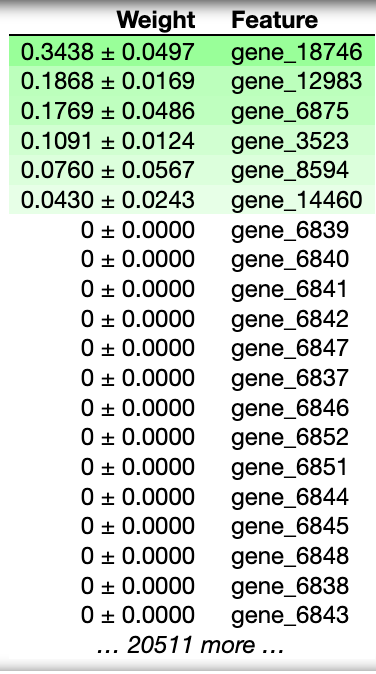
\includegraphics[width=0.2\textwidth]{img/perm}
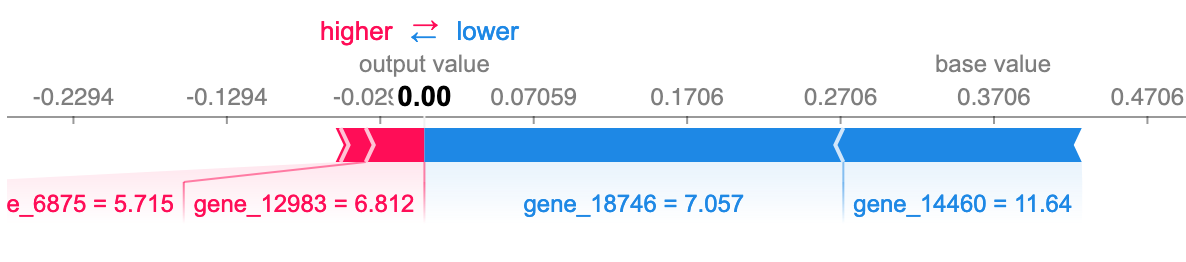
\includegraphics[width=0.77\textwidth]{img/shap.png}
\caption{On the left: permutation importance for the parameter tuned tree. It clearly shows that only a low number of genes is correlated with the prediction. On the right: using Shap library to describe how these features influence data prediction.}
\label{fig_perm}
\end{figure}

We could imagine that only coloured genes were responsible for predictions, so we tried to train a Decision Tree Classifier keeping only those genes. This considerably reduces feature dimensionality, from $20530$ to $6$.The results are:

\begin{figure}[h!]
\centering
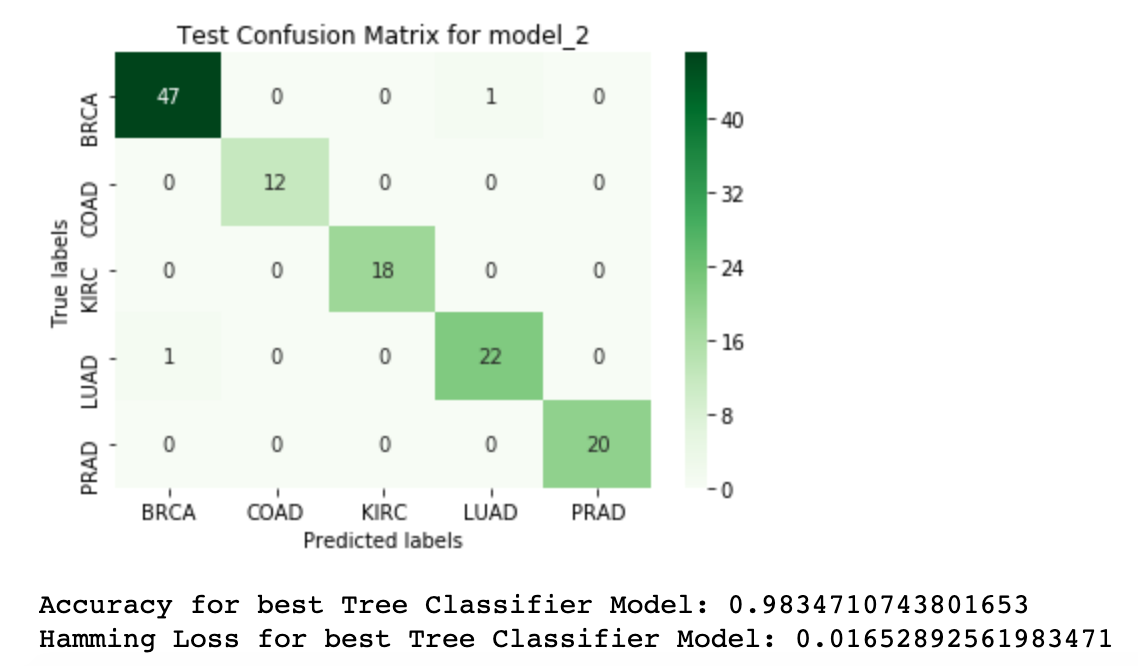
\includegraphics[width=\linewidth]{img/perm_matrix}
\caption{Confusion matrix and evaluation metrics for the tree classifier trained with only "important" genes.}
\label{fig_perm_m}
\end{figure}


%%%%%%%%%%%%%%%%%%%%%%%%%%%%%%%%%%%%%%%%%%%%%%%%%%%%%%%
%%%%%%%%%%%%%%%%%%%%%%%%%%%%%%%%%%%%%%%%%%%%%%%%%%%%%%%

\subsection{Metrics}
During our analysis we used a variety of losses and metrics, for example the already explained Accuracy or the Hamming Loss, which is the fraction of labels that are incorrectly predicted.
Talking about those metrics, we think they are not truly a good measure for nets performances in case of unbalanced classes.
A more precise measure, and the metric we used more often during our work, is the Confusion Matrix.
Having the true labels as rows and predictions as columns, it presents the number of right classifications on the principal diagonal, and the sum of mis-classifications off-diagonal. 
Let's recap our results:
\begin{itemize}
\item For the optimal Decision Tree Classifier, we have and accuracy of $0.9917355371900827 $, a hamming loss of $0.008264462809917356 $ and the model was trained in $3.73$ seconds.
The resulting confusion matrix is:

\begin{figure}[h!]
\centering
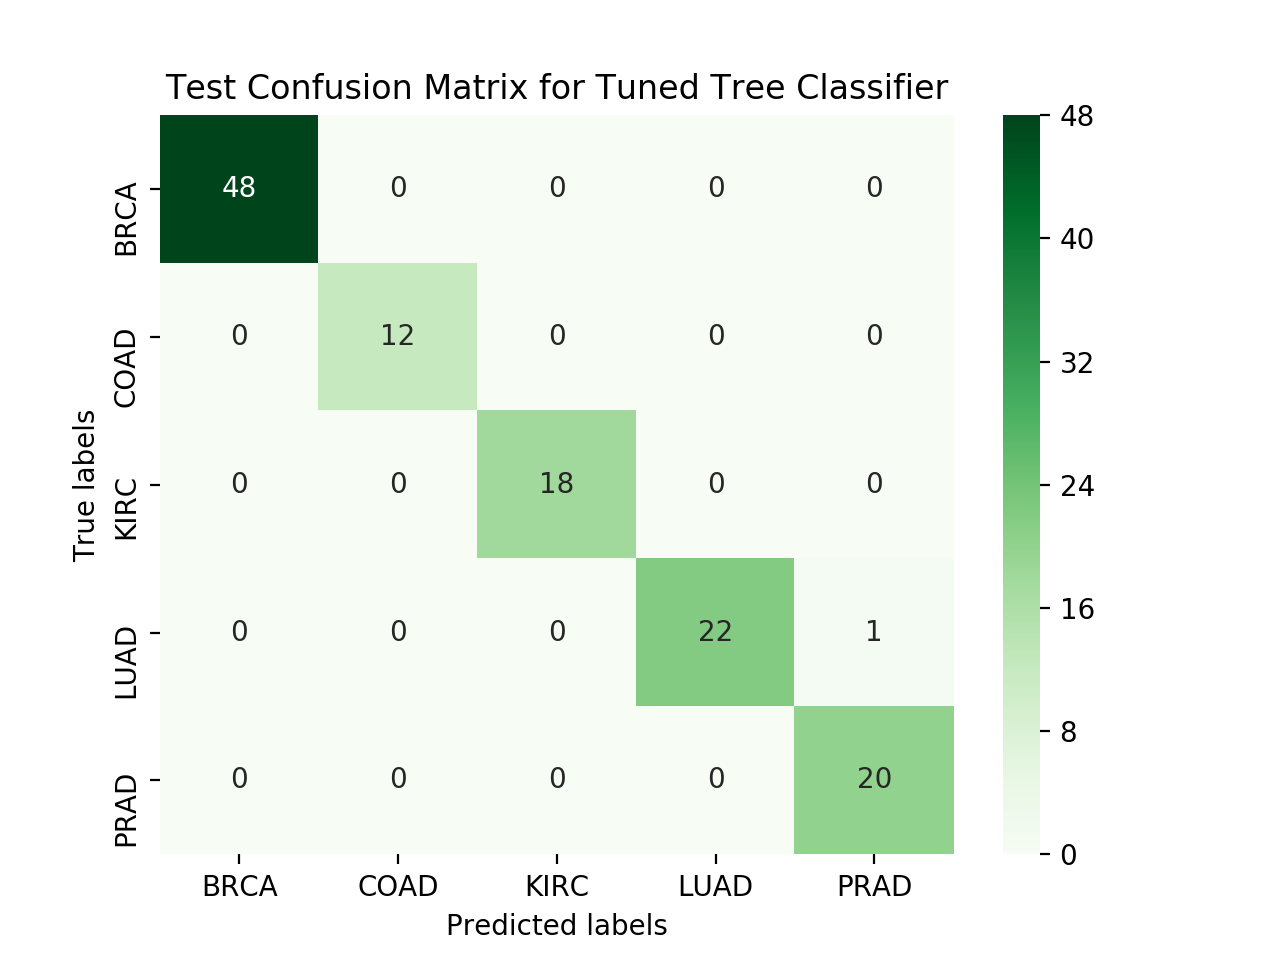
\includegraphics[width=\linewidth]{img/matrix_tree}
\caption{Confusion matrix for the tuned tree classifier.}
\label{mat_tree}
\end{figure}

\item For the optimal Random Forest Classifier, we have and accuracy of $1.0 $, a hamming loss of $0.0$ and the model was trained in $2.37$ seconds. The resulting confusion matrix is:

\begin{figure}[h!]
\centering
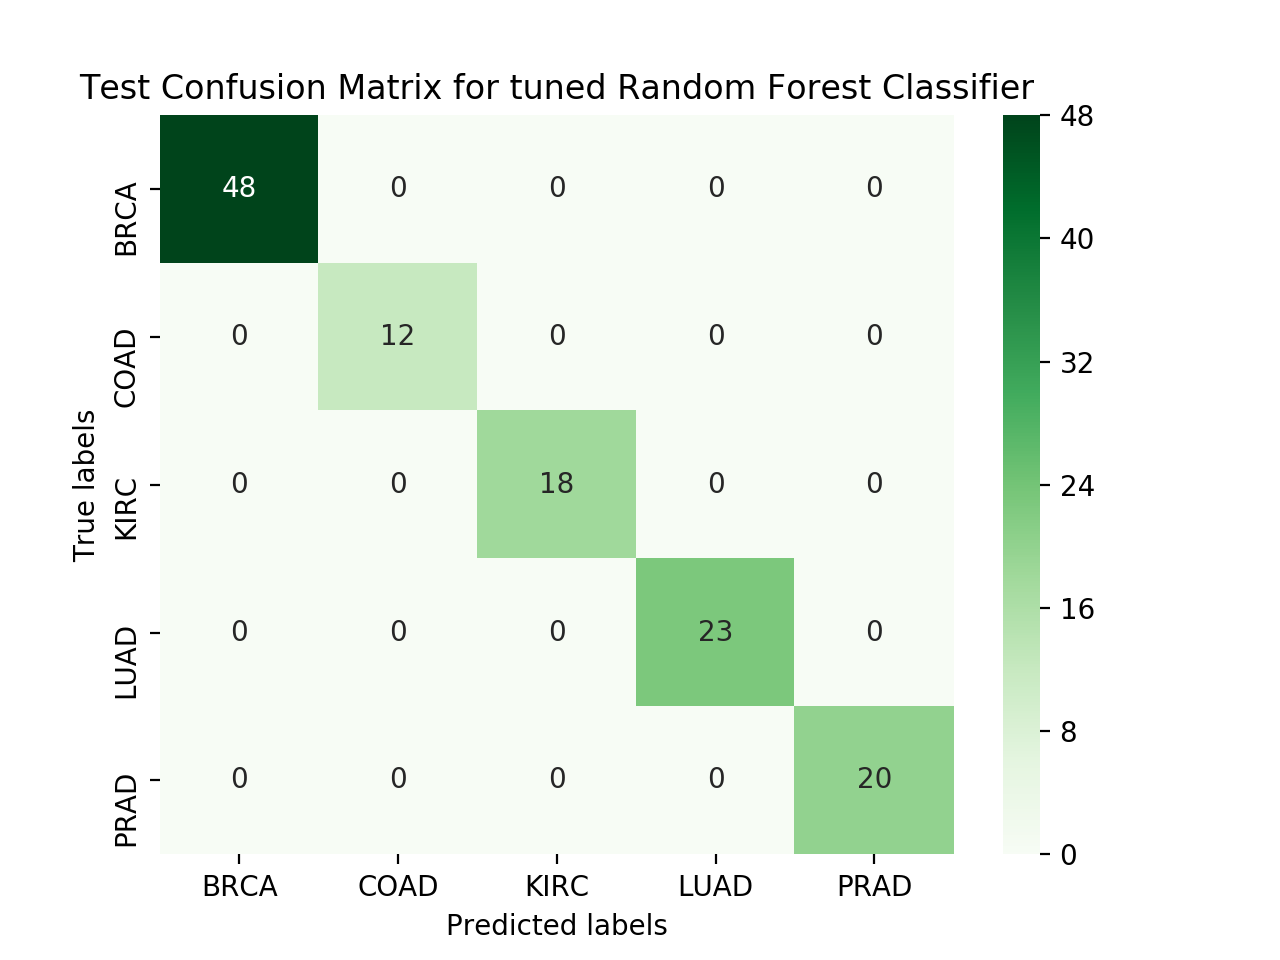
\includegraphics[width=\linewidth]{img/matrix_forest}
\caption{Confusion matrix for the tuned random forest.}
\label{mat_forest}
\end{figure}

\item For the optimal Deep Network with label encoding and CrossEntropyLoss, the model was trained in $21.72$ seconds ending with a CrossEntropyLoss of $0.0000006407485102499777$. The resulting confusion matrix is:


\item For the optimal Deep Network with One-hot Encoding and BCEWithLogitsLoss, the model was trained in $21.21$ seconds ending with a BCEWithLogitsLoss of $0.0054287840612232685$. The resulting confusion matrix is:


\begin{figure}[hbt]
\centering
\advance\leftskip-4cm
\advance\rightskip-4cm
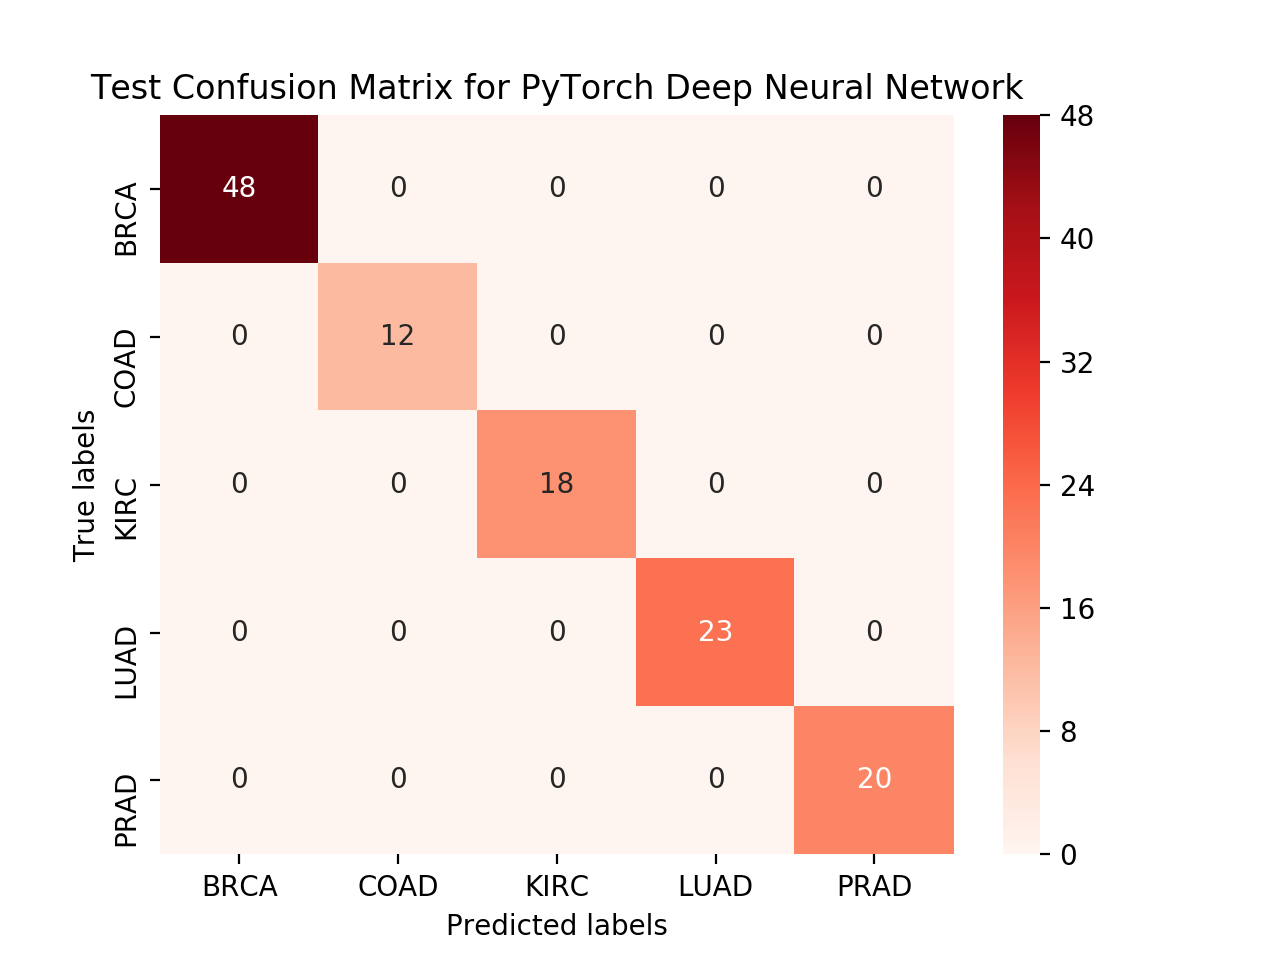
\includegraphics[width=0.7\textwidth]{img/matrix_py_enc}
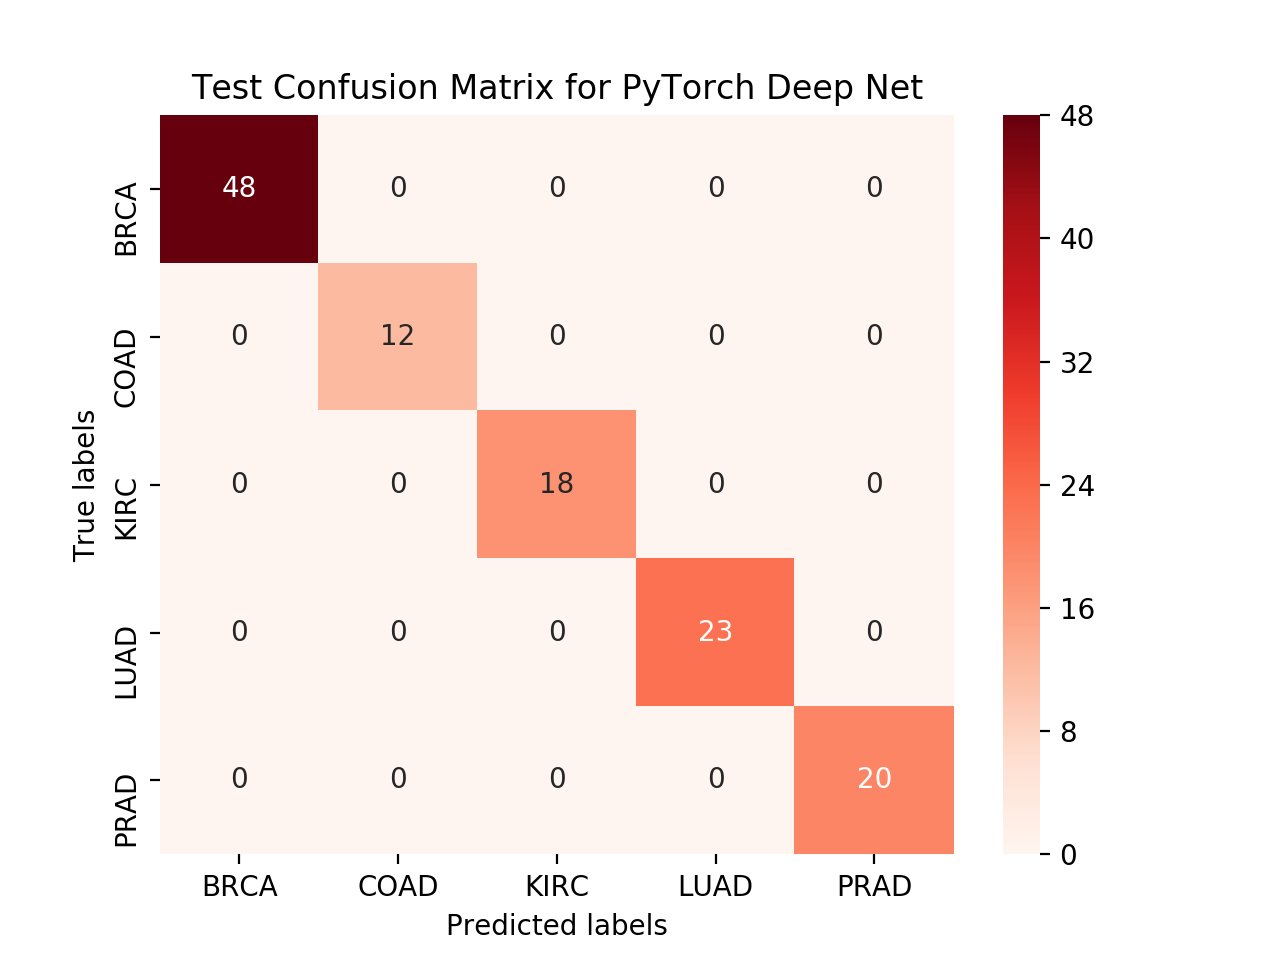
\includegraphics[width=0.7\textwidth]{img/matrix_py_hot}
\caption{On the left: Confusion matrix for the Pytorch Deep Neural Network, with label encoding. On the right: Confusion matrix for the Pytorch Deep Neural Network, with one-hot encoded labels.}
\label{fig_torch}
\end{figure}


\end{itemize}




%%%%%%%%%%%%%%%%%%%%%%%%%%%%%%%%%%%%%%%%%%%%%%%%%%%%%%%
%%%%%%%%%%%%%%%%%%%%%%%%%%%%%%%%%%%%%%%%%%%%%%%%%%%%%%%
%%%%%%%%%%%%%%%%%%%%%%%%%%%%%%%%%%%%%%%%%%%%%%%%%%%%%%%

\section{Conclusions and Outlook}





%%%%%%%%%%%%%%%%%%%%%%%%%%%%%%%%%%%%%%%%%%%%%%%%%%%%%%%
%%%%%%%%%%%%%%%%%%%%%%%%%%%%%%%%%%%%%%%%%%%%%%%%%%%%%%%
%%%%%%%%%%%%%%%%%%%%%%%%%%%%%%%%%%%%%%%%%%%%%%%%%%%%%%%
%%%%%%%%%%%%%%%%%%%%%%%%%%%%%%%%%%%%%%%%%%%%%%%%%%%%%%%


\bibliography{Bibliography}
\bibliographystyle{unsrt}


\end{document}
